\newcommand{\mcol}[3]{\multicolumn{#1}{#2}{#3}}
\newcommand{\mrow}[2]{\multirow{#1}{*}{#2}}
\newcommand{\cellb}{\cellcolor[HTML]{000000}}

\chapter{Metodologi}

Metodologi yang digunakan dalam tugas akhir ini dirancang untuk menyusun, mengimplementasikan, dan mengevaluasi pendekatan berbasis SMT dalam menghitung dimensi metrik dan dimensi metrik sisi suatu graf. Tahapan metodologi ini dibagi menjadi beberapa bagian sebagaimana diilustrasikan oleh \autoref{fig:diagram-alir}.

\begin{figure}[!htbp]
	\centering
	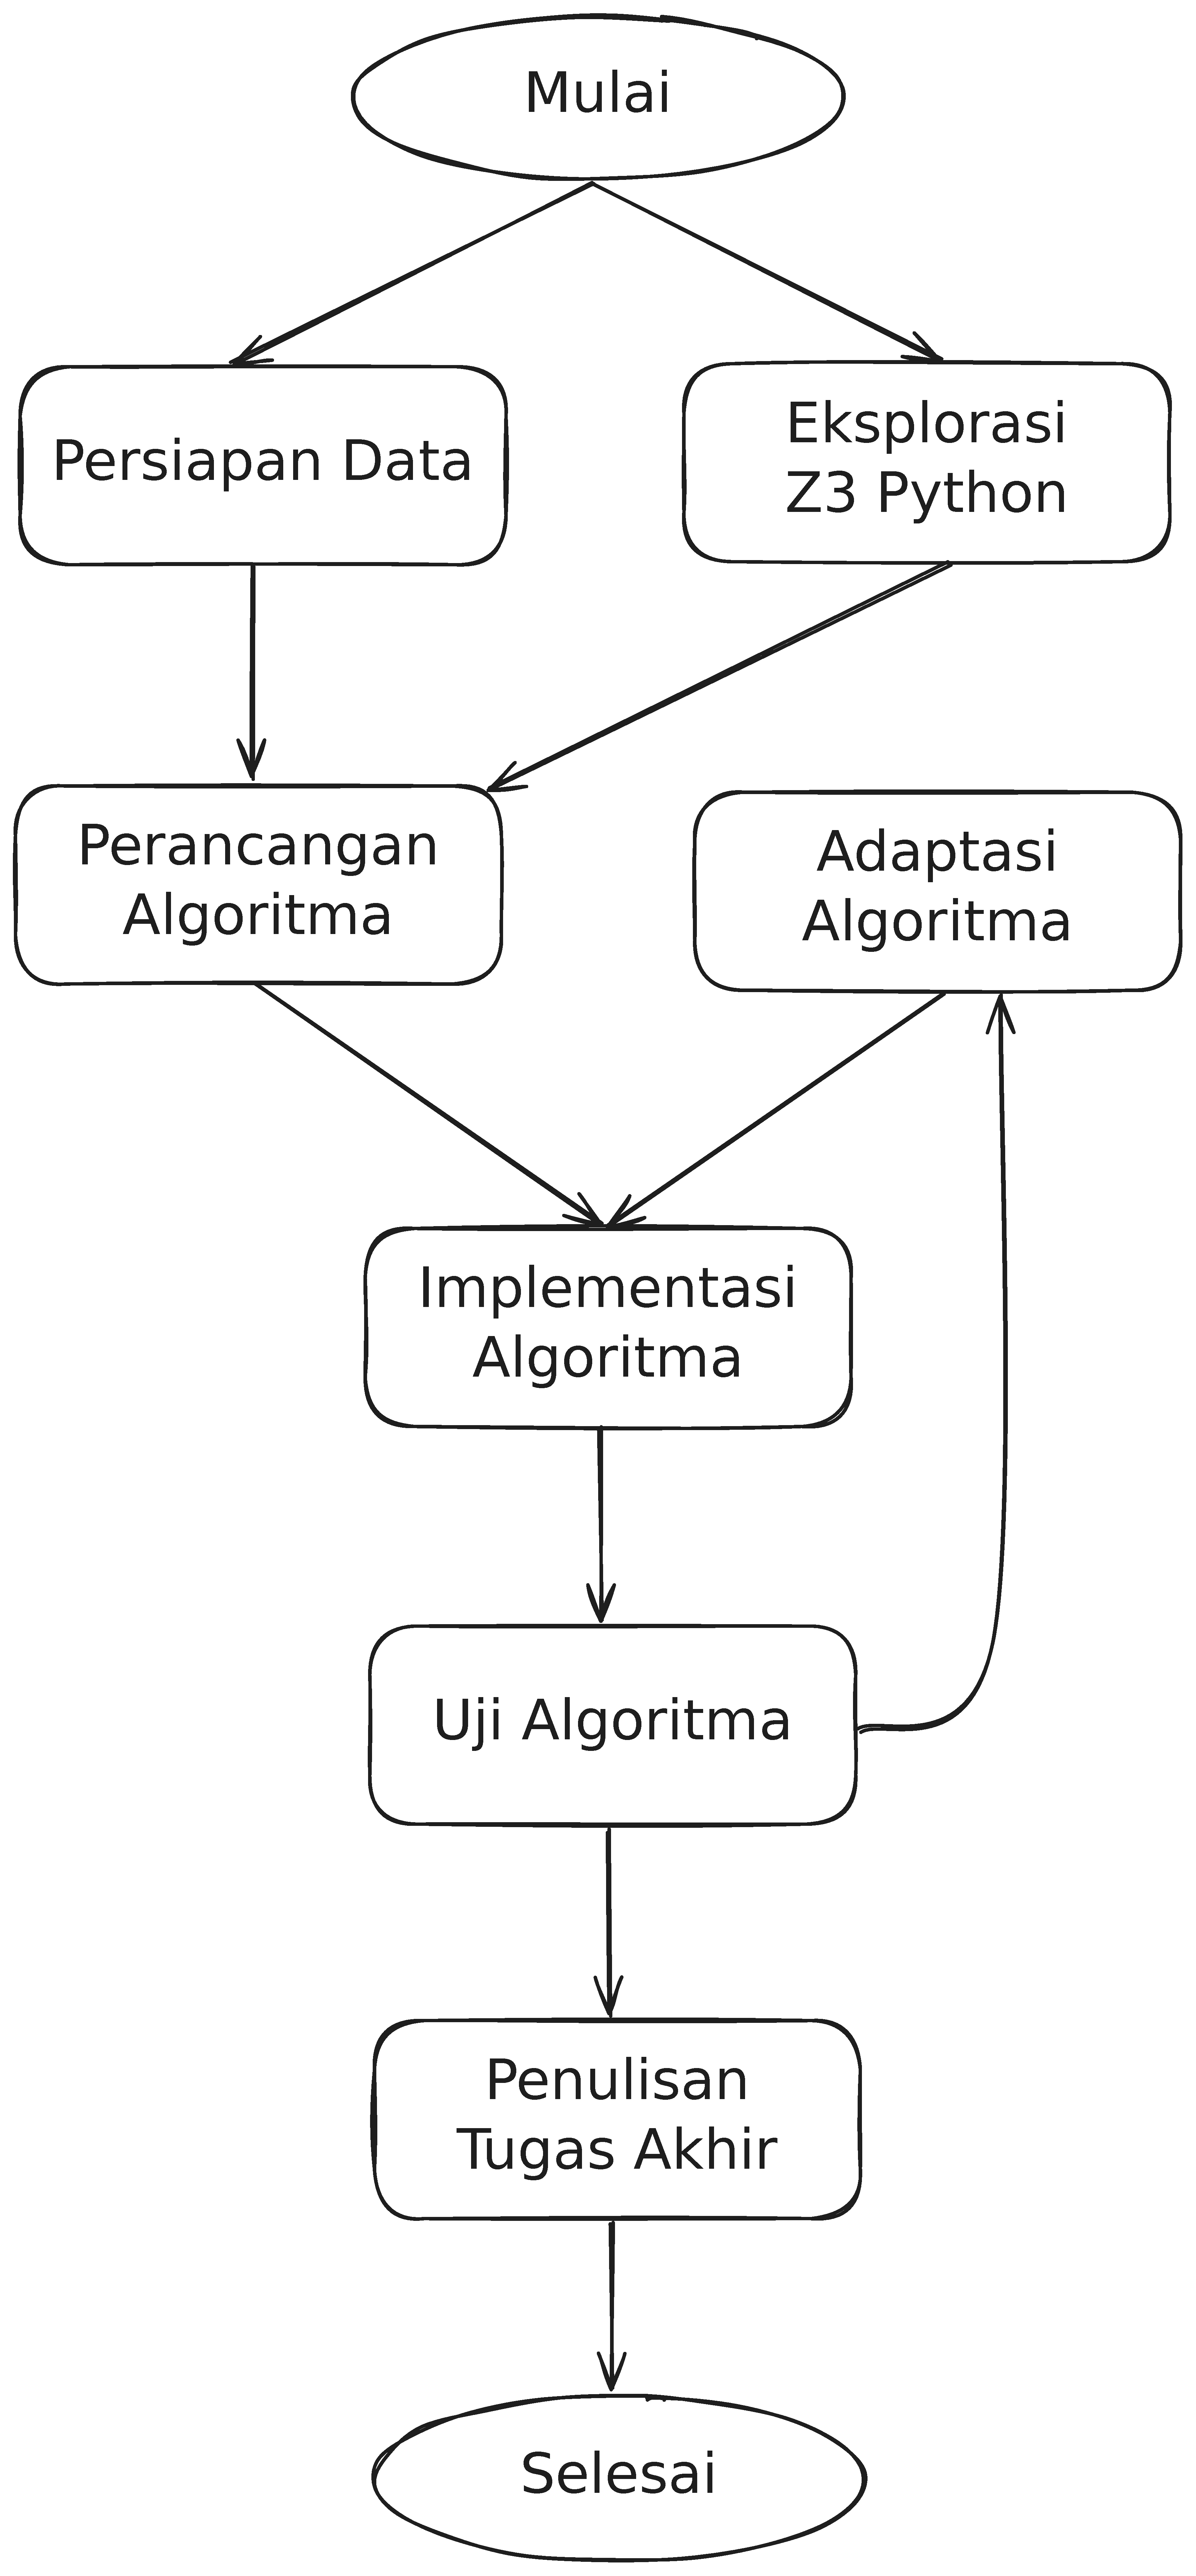
\includegraphics[width=0.5\linewidth]{img/diagram-alir-metodologi.pdf}
	\caption{Diagram Alir Metodologi}
	\label{fig:diagram-alir}
\end{figure}

\clearpage
\section{Persiapan Data}
\label{sec:data}

Data graf yang digunakan dibagi menjadi dua kategori: graf kecil (2 hingga 9 simpul) dan graf besar (lebih dari 9 simpul).

\begin{enumerate}

	\item Graf Kecil

	Graf tak berarah dengan banyak simpul 2 hingga 9 digenerasikan menggunakan program \verb`nauty-geng`. Program ini menghasilkan seluruh graf dengan banyak simpul yang dispesifikasikan dan juga mengeliminasi semua redundansi automorfimanya. Opsi \verb`-c` diberikan kepada program untuk memastikan hanya graf terhubung yang dihasilkan.

	\item Graf Besar

	Graf besar digenerasikan secara acak menggunakan program \verb`nauty-genrang`. Opsi \verb`-g` diberikan kepada program untuk memastikan hanya graf tak berarah yang dihasilkan. Untuk menghindari duplikasi akibat automorfisma, setiap graf diproses menggunakan program \verb`nauty-labelg` untuk menghasilkan representasi kanonik. Kemudian, program \verb`nauty-pickg` dengan opsi \verb`-vc0` digunakan untuk memilih hanya graf yang terkoneksi.

\end{enumerate}

Semua graf disimpan dalam \foreign{file} teks menggunakan format \verb`graph6`. Graf dengan banyak simpul yang sama disimpan dalam file yang sama. Banyak simpul maksimum yang dapat diuji bergantung pada keterbatasan waktu dan sumber daya komputasi yang tersedia.

\section{Eksplorasi Z3 Python}

Pada tahap ini dilakukan eksplorasi SMT \foreign{solver}, yaitu Z3, menggunakan \foreign{binding} untuk bahasa Python. Aktivitas meliputi:

\begin{enumerate}

	\item Mempelajari fitur dasar Z3 yang relevan dengan formulasi masalah kombinatorial pada teori graf.

	\item Mencoba contoh sederhana untuk memahami cara mendefinisikan variabel, batasan (\foreign{constraints}), serta strategi pencarian solusi.

	\item Mengevaluasi kemampuan Z3 dalam menangani permasalahan berukuran kecil maupun besar untuk mengidentifikasi potensi kendala performa.

\end{enumerate}

\section{Perancangan Algoritma}

Perancangan algoritma difokuskan pada formulasi masalah dimensi metrik ke dalam bentuk SMT. Pertama, graf direpresentasikan dalam bentuk matriks ketetanggaan yang dibaca dari format \verb`graph6`. Kedua, matriks jarak dapat dibangun dari matriks ketetanggaan menggunakan algoritma \foreign{Floyd–Warshall}. Kemudian, berdasarkan dua informasi ini, dirancanglah algoritma yang memetakan pencarian dimensi metrik ke dalam bentuk batasan yang dapat dicerna oleh SMT.

Dalam tugas akhir ini, digunakan tiga teori dalam SMT, yaitu \foreign{boolean satisfiability}, \foreign{pseudo boolean}, dan \foreign{linear integer arithmetic}. Dipilih teori \foreign{boolean satisfiability} karena permasalahan dimensi metrik yang perlu memodelkan \foreign{resolving set}, yaitu memilih keanggotaan simpul graf yang dapat dinyatakan menggunakan \foreign{constraints} boolean. Sedangkan teori \foreign{pseudo boolean} serta \foreign{linear integer arithmetic} dipilih sebagai eksplorasi tambahan mengenai kapabilitas SMT, karena translasi \foreign{constraint} dari \foreign{boolean satisfiability} ke dalam kedua teori ini yang masih cukup mudah untuk dilakukan.

\section{Implementasi Algoritma}

Algoritma yang telah dirancang kemudian diimplementasikan ke bentuk kode. Hal-hal yang perlu dilakukan diantaranya adalah:

\begin{enumerate}

		\item Pembacaan graf dari \foreign{file} teks \verb`graph6`.

		\item Formulasi batasan untuk SMT dari informasi graf.

		\item Eksekusi Z3 \foreign{solver} dan dapatkan dimensi metrik.

		\item Simpan hasil perhitungan ke dalam \foreign{file} teks untuk analisis lebih lanjut.

\end{enumerate}

\section{Uji Algoritma}

Pengujian dilakukan secara bertahap untuk memverifikasi kebenaran implementasi serta mengevaluasi kinerjanya.

\begin{enumerate}

	\item{Uji pada Sampel Kecil}

	Beberapa graf kecil dipilih sebagai sampel. Tujuan tahap pengujian ini adalah memverifikasi bahwa rancangan algoritma dan implementasi program menghasilkan solusi yang benar.

	\item{Uji pada Seluruh Graf Kecil}

	Seluruh graf terhubung dengan 2–9 simpul diuji secara menyeluruh. Tujuan tahap pengujian ini adalah untuk mendapatkan data komprehensif kinerja algoritma dengan berbagai macam konfigurasi graf. Data ini dapat dianalisis kasus-kasusnya seperti kejadian \foreign{worst-case} dan kejadian \foreign{best-case}. Hasil ini juga dapat dibandingkan dengan literatur yang ada untuk validasi.

	\item{Uji pada Graf Besar}

	Pengujian diperluas pada graf dengan simpul lebih banyak. Tujuan tahap pengujian ini adalah mengevaluasi kinerja dan keterbatasan pendekatan SMT pada kasus yang lebih kompleks. Uji ini juga yang dijadikan sebagai tolak ukur performa solusi dari tugas akhir ini secara umum untuk sembarang graf.

\end{enumerate}

\section{Adaptasi Algoritma}

Tahap adaptasi dilakukan dengan memodifikasi algoritma yang telah ada untuk menghitung dimensi metrik sisi. Proses adaptasi mencakup:

\begin{enumerate}

	\item Menyesuaikan representasi graf sehingga memperhatikan jarak antar sisi.

	\item Memformulasikan kembali permasalahan ke dalam SMT.

	\item Mengimplementasikan kembali ke bentuk kode.

	\item Mengulangi tahapan pengujian: mulai dari sampel kecil, seluruh graf kecil, hingga graf besar.

\end{enumerate}

\section{Penulisan Tugas Akhir}

Tahap terakhir dari metodologi ini adalah penyusunan seluruh hasil penelitian ke dalam bentuk laporan tugas akhir. Penulisan dilakukan sesuai pedoman akademik yang berlaku sehingga hasil penelitian terdokumentasi dengan baik dan dapat dijadikan rujukan untuk penelitian selanjutnya.
